\documentclass[11pt]{article}

\usepackage[T1]{fontenc}
\usepackage{newtxtext}
\usepackage[margin=1in]{geometry}
\usepackage{microtype}
\usepackage{amsmath}
\usepackage{newtxmath}
\usepackage{booktabs}
\usepackage{graphicx}
\usepackage{xcolor}
\usepackage[numbers,sort&compress]{natbib}
\usepackage{caption}
\usepackage{enumitem}
\usepackage{listings}
\usepackage{tikz}
\usetikzlibrary{arrows.meta,positioning,fit,calc}
\usepackage[colorlinks=true,linkcolor=ourblue,citecolor=ourblue,urlcolor=ourblue]{hyperref}

\definecolor{ourblue}{HTML}{0F4D92}
\definecolor{ourred}{HTML}{B64342}
\definecolor{ourgrey}{HTML}{767676}
\definecolor{lightblue}{HTML}{DCE8F5}
\definecolor{lightred}{HTML}{F6CFCB}

\captionsetup{font=small,labelfont=bf}
\setlist{itemsep=2pt,topsep=4pt}
\lstset{basicstyle=\ttfamily\footnotesize,breaklines=true,frame=single,columns=fullflexible,
        backgroundcolor=\color{black!3},rulecolor=\color{black!25}}

\newcommand{\plain}{\textsc{Plain}}
\newcommand{\indep}{\textsc{Independent}}
\newcommand{\ordered}{\textsc{Ordered}}
\newcommand{\todo}[1]{\textcolor{ourred}{[TODO: #1]}}

\title{\textbf{Where Did the Tokens Go?}\\[4pt]
\large Build Order in Hierarchical Code Generation, and a Blind Spot in Token-Budget Evaluation}
\author{Animesh Ratna\\[2pt]
{\normalsize BITS Pilani}\\[1pt]
{\normalsize\texttt{f20240665@pilani.bits-pilani.ac.in}}}
\date{November 2026}

\begin{document}
\maketitle

\begin{abstract}
A large language model can write a program in one go, or split the problem into small functions, write each function
separately, and assemble the pieces. DecompRL, a recent reinforcement-learning method, takes the second route and
writes every function independently, seeing only the other functions' names and descriptions. We ask whether the
\emph{order} in which the functions are built matters, before any training. Our method, ordered decomposition, builds
the simplest functions first and shows each later function the finished code of the functions it calls.
On 279 competitive-programming problems from LiveCodeBench, with Qwen2.5-7B-Instruct and DecompRL's own evaluation
rule (the share of problems solved within a fixed budget of generated tokens), ordered decomposition beats independent
decomposition at a budget of 50,000 tokens per problem: 0.237 against 0.165, a paired difference of $+0.072$ (95\%
confidence interval $[+0.032, +0.111]$). This was our pre-registered primary test.
The gain does not come from better attempts: attempt for attempt, the two methods tie. It comes from cheaper ones.
Seeing finished code lets each function reuse it instead of rewriting it, so an ordered attempt generates a third as
many tokens and the same budget buys four times as many attempts. But the reused code is read as input, which the
budget does not count. Counting input tokens reverses the result, and measured in GPU time the gain shrinks to
$+0.028$ ($[-0.006, +0.062]$). Sampling whole programs, with no decomposition at all, beats both methods.
We recommend that budget-based evaluations of code generation report input tokens and GPU time alongside generated
tokens. Code and the full run record: \url{https://github.com/RatnaAnimesh/build-order-codegen}.
\end{abstract}

% =====================================================================================================================
\section{Introduction}

Language models that write code are usually allowed several tries. Every try is checked against hidden tests, and the
problem counts as solved if any try passes. Because tries are cheap to check, a method can trade quality for quantity:
it can make each try worse and still win by making more of them. A fair comparison therefore fixes a budget per
problem and asks how much each method solves within it. DecompRL~\citep{decugis2026decomprl} counts that budget in
\emph{generated tokens}, the words and symbols the model writes, and calls the resulting score pass@tokens.

DecompRL generates code hierarchically. One call to the model splits a problem into at most six functions and writes
only their signatures and short descriptions (``stubs''). Further calls then write eight versions of each function's
body, each one seeing only the stubs of the others. Choosing one version of every function gives up to $8^n$ different
programs, and the problem is solved if any of them passes. The authors train both steps with reinforcement learning
on 80 H100 GPUs for two to three days per run, and report that on LiveCodeBench~\citep{jain2024livecodebench}
the trained Qwen2.5-7B model beats a standard reinforcement-learning baseline (GRPO,~\citep{shao2024deepseekmath})
from 50,000 tokens per problem upward, while trailing it at 5,000 and 10,000.

Writing every function independently is a design choice, and the paper names its cost: a function is written without
seeing the code it will call. Human programmers often work the other way round. They write the small pieces first
and build larger pieces on top of code that already exists. This paper asks a narrow question: \emph{on DecompRL's
own benchmark, model and metric, does building functions in dependency order change what hierarchical generation
buys?} We answer it at inference time, on the same untrained model, so that a difference cannot come from training.

We compare three ways of spending a token budget (Section~\ref{sec:methods}): sampling whole programs (\plain),
DecompRL's inference procedure (\indep), and our ordered variant (\ordered). We fixed the analysis in writing before
the full run. We find:
\begin{enumerate}[label=(\arabic*)]
  \item \textbf{\ordered{} beats \indep{} on the paper's metric.} At 50,000 generated tokens per problem it solves
        0.237 of problems against 0.165, a paired difference of $+0.072$ $[+0.032, +0.111]$.
  \item \textbf{The attempts are not better, only cheaper.} With one attempt each the two methods tie. An \ordered{}
        attempt generates 5,573 tokens against 17,032, so the budget buys 8 attempts instead of 2.
  \item \textbf{The saving moves into the input.} An \ordered{} attempt reads 43,779 input tokens against 5,980.
        Counting input tokens reverses the order, and in GPU time the difference is not significant.
  \item \textbf{Neither beats plain sampling.} \plain{} reaches 0.312 at 10,000 tokens, above both decomposition
        methods at 50,000.
\end{enumerate}
The general lesson is about measurement. A budget in generated tokens rewards any method that moves work from what
the model writes into what it reads. We argue that such evaluations should report all three costs: generated tokens,
input tokens and GPU time.

\paragraph{Scope.} We train neither method. This paper compares inference procedures on one untrained model; it does
not compare against the reinforcement-learning-trained DecompRL model, and it makes no claim to beat it.

% =====================================================================================================================
\section{Background}
\label{sec:background}

\paragraph{Judging generated code.} A competitive-programming problem comes with hidden tests. A program counts as
correct only if it passes all of them within a time limit. LiveCodeBench~\citep{jain2024livecodebench} collects such
problems from contests on AtCoder and LeetCode and dates each one, so that a model can be tested on problems published
after its training data was collected.

\paragraph{Attempts and pass@$k$.} Models sample their output at random, so each try at a problem (an
\emph{attempt}) can turn out differently. pass@$k$ is the chance that at least one of $k$ attempts is correct.
Given $n$ attempts of which $c$ passed, the unbiased estimate~\citep{chen2021codex} is
\begin{equation}
  \text{pass@}k \;=\; 1 - \binom{n-c}{k} \Big/ \binom{n}{k}, \qquad k \le n,
  \label{eq:passk}
\end{equation}
averaged over problems.

\paragraph{Budgets: pass@tokens.} Attempts of different methods cost different amounts: a whole program might be 300
tokens, a decomposed attempt 17,000. DecompRL (its Appendix K) therefore converts a budget of $B$ tokens into a number
of attempts,
\begin{equation}
  k \;=\; \max\!\left(1, \left\lfloor B / \bar c \right\rfloor\right),
  \label{eq:budget}
\end{equation}
where $\bar c$ is the method's mean number of generated tokens per attempt, and reports pass@$k$. A method whose
attempts cost 4,000 tokens thus gets two attempts from a 10,000-token budget. We call this score pass@tokens.

\paragraph{What a token costs.} A model reads its input (the \emph{prompt}) all at once, in parallel, a step called
prefill; it then writes its output one token at a time, a step called decoding~\citep{pope2023inference}. Per token,
reading is much cheaper than writing, but it is not free, and a prompt tens of thousands of tokens long takes real
GPU time. pass@tokens counts only the written tokens. We therefore also measure budgets in GPU-seconds.

% =====================================================================================================================
\section{The three methods}
\label{sec:methods}

\begin{figure}[t]
\centering
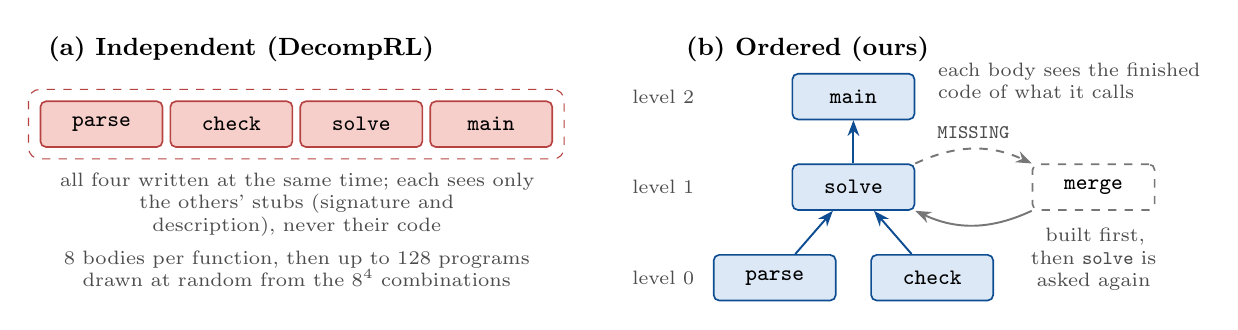
\begin{tikzpicture}[font=\footnotesize,
  fn/.style={draw, rounded corners=2pt, minimum width=1.55cm, minimum height=0.58cm, fill=white, line width=0.6pt},
  done/.style={fn, fill=lightblue, draw=ourblue},
  stub/.style={fn, fill=lightred, draw=ourred},
  arr/.style={-{Stealth[length=2mm]}, line width=0.7pt},
  lab/.style={font=\scriptsize, text=black!70, align=center}]
% ---------- (a) Independent
\node[font=\small\bfseries, anchor=west] at (-0.2, 3.35) {(a) Independent (DecompRL)};
\node[stub] (ip) at (0.6, 2.4) {\texttt{parse}};
\node[stub] (ic) at (2.25, 2.4) {\texttt{check}};
\node[stub] (is) at (3.9, 2.4) {\texttt{solve}};
\node[stub] (im) at (5.55, 2.4) {\texttt{main}};
\node[draw, dashed, rounded corners, fit=(ip)(im), inner sep=4pt, draw=ourred] {};
\node[lab, anchor=north, text width=6.6cm] at (3.08, 1.9) {all four written at the same time; each sees only\\
  the others' stubs (signature and description), never their code\\[4pt]
  8 bodies per function, then up to 128 programs\\ drawn at random from the $8^4$ combinations};
% ---------- (b) Ordered
\begin{scope}[xshift=8.5cm]
\node[font=\small\bfseries, anchor=west] at (-0.6, 3.35) {(b) Ordered (ours)};
\node[lab, anchor=east] at (-0.25, 0.45) {level 0}; \node[lab, anchor=east] at (-0.25, 1.6) {level 1};
\node[lab, anchor=east] at (-0.25, 2.75) {level 2};
\node[done] (op) at (0.65, 0.45) {\texttt{parse}};
\node[done] (oc) at (2.65, 0.45) {\texttt{check}};
\node[done] (os) at (1.65, 1.6) {\texttt{solve}};
\node[done] (om) at (1.65, 2.75) {\texttt{main}};
\node[fn, dashed, draw=ourgrey] (oh) at (4.7, 1.6) {\texttt{merge}};
\draw[arr, ourblue] (op) -- (os); \draw[arr, ourblue] (oc) -- (os); \draw[arr, ourblue] (os) -- (om);
\draw[arr, ourgrey, dashed] (os.north east) to[bend left=25] node[lab, above] {\texttt{MISSING}} (oh.north west);
\draw[arr, ourgrey] (oh.south west) to[bend left=25] (os.south east);
\node[lab, anchor=north, text width=2.3cm] at (4.7, 1.2) {built first, then \texttt{solve} is asked again};
\node[lab, anchor=west, align=left] at (2.6, 2.95) {each body sees the finished\\ code of what it calls};
\end{scope}
\end{tikzpicture}
\caption{How one attempt builds a program with four functions. \textbf{(a)}~\indep{} writes every function at once,
from stubs only. \textbf{(b)}~\ordered{} builds functions level by level, simplest first; each body is shown finished
code for the functions it calls (blue arrows), and may ask for a helper the plan forgot (\texttt{MISSING}).}
\label{fig:methods}
\end{figure}

All three methods use the same model, the same sampling settings and the same tests. They differ only in what each
model call sees and in what order the calls are made (Figure~\ref{fig:methods}).

\paragraph{\plain: sampling whole programs.} The model sees the problem in LiveCodeBench's standard prompt and writes
a complete program. One attempt is one program.

\paragraph{\indep: DecompRL's inference procedure.} One call writes a \emph{decomposition}: up to six functions, each
with a type signature and a description, and an empty body. For each function the model then writes eight bodies, each
from the problem and all the stubs. A program takes one body per function. Up to 128 programs are drawn uniformly at
random from all combinations, and the attempt succeeds if any of them passes every test. We use DecompRL's prompts
(its Appendix~I) unchanged.

\paragraph{\ordered: our variant.} We make three changes to DecompRL's prompts and nothing else.
\begin{enumerate}[label=(\roman*)]
  \item \emph{The plan names dependencies.} Each description ends with a line \texttt{Uses: f, g} naming the functions
        it calls, and functions are listed simplest first.
  \item \emph{Functions are built in levels.} Functions that call no other function are built first, then those whose
        callees are all built, and so on. Each of a function's eight bodies is shown one finished body, picked at
        random, for every function it calls, in place of that function's stub.
  \item \emph{Missing pieces are asked for, not invented.} A body may reply \texttt{MISSING:} with the signature and
        purpose of a helper the plan forgot, instead of calling a function that does not exist. The helper is built
        and the body is asked again, at most twice. A static check also catches calls to undefined functions and
        builds those helpers.
\end{enumerate}
Programs are assembled the same way as in \indep, except that the first eight are \emph{coherent}: each pairs a
top-level body with exactly the callee bodies it was shown while being written. Random combinations then fill the
remaining slots up to 128.

\paragraph{Shared rules.} Every generated token counts against the attempt that caused it, including \texttt{MISSING}
replies, helpers and repeated requests. A decomposition with more than six functions, or one that cannot be parsed,
fails the attempt; this is DecompRL's limit and applies to both decomposition methods.
Table~\ref{tab:cost} lists what one attempt cost in our run.

\begin{table}[t]
\centering
\caption{The cost of one attempt, averaged over all attempts of the main run. GPU-seconds are generation wall time on
two T4 GPUs, input processing included, divided by the number of attempts.}
\label{tab:cost}
\begin{tabular}{lrrrr}
\toprule
 & Generated tokens & Input tokens & GPU-seconds & Attempts made \\
\midrule
\plain{}  & 260    & 33     & 0.4  & 10,602 \\
\indep{}  & 17,032 & 5,980  & 26.8 & 558 \\
\ordered{} & 5,573 & 43,779 & 16.4 & 2,232 \\
\bottomrule
\end{tabular}
\end{table}

% =====================================================================================================================
\section{Experimental setup}
\label{sec:setup}

\paragraph{Model and hardware.} Qwen2.5-7B-Instruct~\citep{qwen2024qwen25} in 16-bit precision, served with vLLM
0.8.5~\citep{kwon2023vllm} across two NVIDIA T4 GPUs (16\,GB each) on Kaggle's free tier, with an 8,192-token context.
Sampling uses temperature 1.0 and top-$p$ 1.0, DecompRL's evaluation setting.

\paragraph{Problems.} The LiveCodeBench problems dated 1 August 2024 to 1 February 2025, the window DecompRL evaluates
on: 279 problems, 175 from AtCoder (read input, print output) and 104 from LeetCode (complete a given function).
LiveCodeBench labels 67 as easy, 89 as medium and 123 as hard.

\paragraph{Grading.} Programs run in a sandbox with memory and file-size limits, against each problem's public tests
and then its private tests, stopping at the first failure. The time limit is DecompRL's, $2T + 1$ seconds for $T$
tests, measured as CPU time because the grader shared its CPUs with the model server. Outputs are compared with
LiveCodeBench's rules.

\paragraph{Sampling schedule.} The run proceeds in rounds with a rising target budget per problem: 5k, 10k, 20k, 30k,
40k and 50k generated tokens. Each round tops every problem up, method by method, to the number of attempts that budget
buys under Equation~\eqref{eq:budget}. \plain{} is sampled only up to 10k, the range of the sanity check below. The run took three sessions (9.67, 2.61 and 3.78 hours), generated 24.7 million tokens from 101.4
million input tokens, and left no attempt ungraded.

\paragraph{Pre-registered analysis.} Before the full run we fixed in writing:
\begin{enumerate}[label=(\arabic*)]
  \item \emph{Sanity check}: \plain{} within 0.05 of DecompRL's untrained baseline (its Table~1) at 5k and 10k tokens.
  \item \emph{Primary test}: \ordered{} minus \indep{} at the largest budget both cover. \ordered{} wins if the 95\%
        confidence interval lies above zero.
  \item \emph{Secondary tests}: each decomposition method minus \plain{} at the largest budget all three cover, and
        \indep{} minus \plain{} at 4k tokens, where DecompRL's Table~4 reports $-3$ points.
\end{enumerate}
A method \emph{covers} a budget if at least 95\% of problems have the $k$ graded attempts that budget buys. Every
difference is paired by problem; its confidence interval is a percentile bootstrap over problems with 4,000 resamples
\citep{efron1994bootstrap}. Analyses not on this list are marked as added after the run.

% =====================================================================================================================
\section{Results}
\label{sec:results}

\begin{figure}[t]
\centering
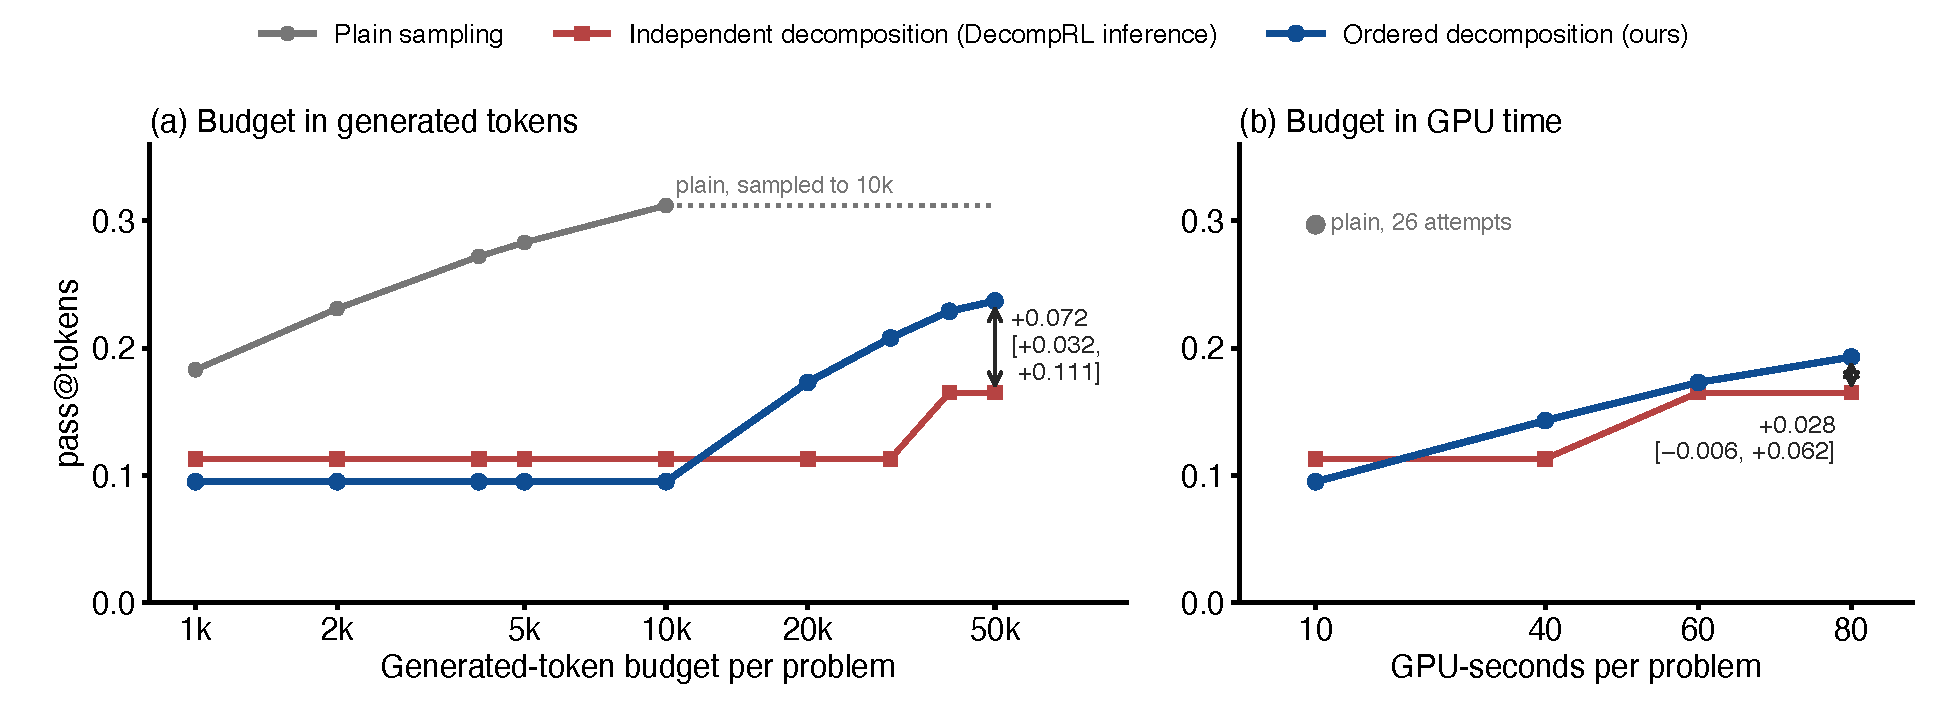
\includegraphics[width=\linewidth]{figures/pass_at_budget.pdf}
\caption{Share of problems solved as the budget per problem grows. \textbf{(a)}~Budget in generated tokens, DecompRL's
metric: \ordered{} overtakes \indep{} once the budget buys it more than one attempt, and leads by 0.072 at 50k; \plain{}
(sampled up to 10k) stays above both. \textbf{(b)}~The same attempts with GPU-seconds as the price: the lead at 80
GPU-seconds, the largest budget both decomposition methods cover, is not significant. Brackets give 95\% confidence
intervals for the paired difference.}
\label{fig:budget}
\end{figure}

\paragraph{The primary test passes.} Figure~\ref{fig:budget}(a) shows each method's score as the token budget grows.
Both decomposition methods cover budgets up to 50k tokens, and there \ordered{} solves 0.237 of problems against
\indep's 0.165. The paired difference is $+0.072$ with a 95\% interval of $[+0.032, +0.111]$, entirely above zero
(Table~\ref{tab:tests}). Up to 10k each decomposition method can afford only one attempt, and there \indep{} is
slightly ahead (0.113 against 0.095).

\paragraph{Plain sampling beats both.} All three methods cover 10k tokens. There \plain{}, with 38 attempts per problem,
solves 0.312, about 0.2 more than either decomposition method (Table~\ref{tab:tests}). \plain{} at 10k is also above
both decomposition methods at 50k. On an untrained model, decomposing is a worse use of tokens than sampling whole
programs.

\begin{table}[t]
\centering
\caption{Paired differences in pass@tokens, with 95\% bootstrap confidence intervals over the 279 problems.}
\label{tab:tests}
\small
\begin{tabular}{llrl}
\toprule
Comparison & Budget & Difference [95\% CI] & Status \\
\midrule
\ordered{} $-$ \indep{} (primary) & 50k tokens & $+0.072$ $[+0.032, +0.111]$ & pre-registered \\
\ordered{} $-$ \plain{} & 10k tokens & $-0.217$ $[-0.261, -0.173]$ & pre-registered \\
\indep{} $-$ \plain{} & 10k tokens & $-0.199$ $[-0.247, -0.152]$ & pre-registered \\
\indep{} $-$ \plain{} (DecompRL: $-0.03$) & 4k tokens & $-0.159$ $[-0.202, -0.119]$ & pre-registered \\
\midrule
\ordered{} $-$ \indep{}, one attempt each & $\le$10k tokens & $-0.018$ $[-0.041, +0.004]$ & after the run \\
\ordered{} $-$ \indep{} & 80 GPU-s & $+0.028$ $[-0.006, +0.062]$ & after the run \\
\bottomrule
\end{tabular}
\end{table}

\paragraph{By difficulty.} At 50k tokens \ordered{} leads at every difficulty level (Figure~\ref{fig:difficulty}). Hard
problems stay almost unsolved by both: \ordered{} solves 0.024 of the 123 hard problems and \indep{} none.

\begin{figure}[t]
\centering
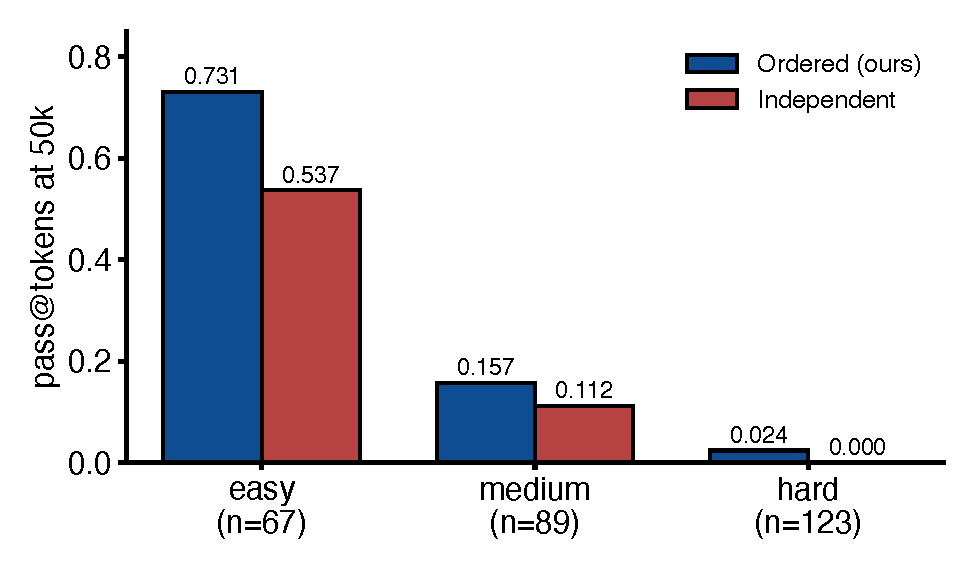
\includegraphics[width=0.55\linewidth]{figures/by_difficulty.pdf}
\caption{pass@tokens at 50k generated tokens by LiveCodeBench difficulty label.}
\label{fig:difficulty}
\end{figure}

% =====================================================================================================================
\section{Where the gain comes from}
\label{sec:analysis}

All analyses in this section were added after the run.

\paragraph{Not better attempts.} With exactly one attempt each, the two decomposition methods tie: \ordered{} minus
\indep{} is $-0.018$ $[-0.041, +0.004]$. \ordered's plans also fail more often before any code is written: 287 of its
2,232 decompositions (12.9\%) were unusable, 149 for exceeding six functions and 138 for being unparseable, against 45
of \indep's 558 (8.1\%). Its plans did follow the new format: 97\% of its decompositions carried \texttt{Uses:} lines,
with 2.4 dependency levels on average.

\paragraph{Cheaper attempts.} Both methods write about 29 function bodies per attempt. \ordered's bodies average about
190 tokens against \indep's 580, because a body that can see the finished code of a function simply calls it, where
a body that sees only a stub tends to re-implement what it needs. An \ordered{} attempt therefore generates a third of
the tokens (5,573 against 17,032), and a 50k budget buys it 8 attempts against \indep's 2. The win in
Figure~\ref{fig:budget}(a) comes from those extra attempts.

\begin{figure}[t]
\centering
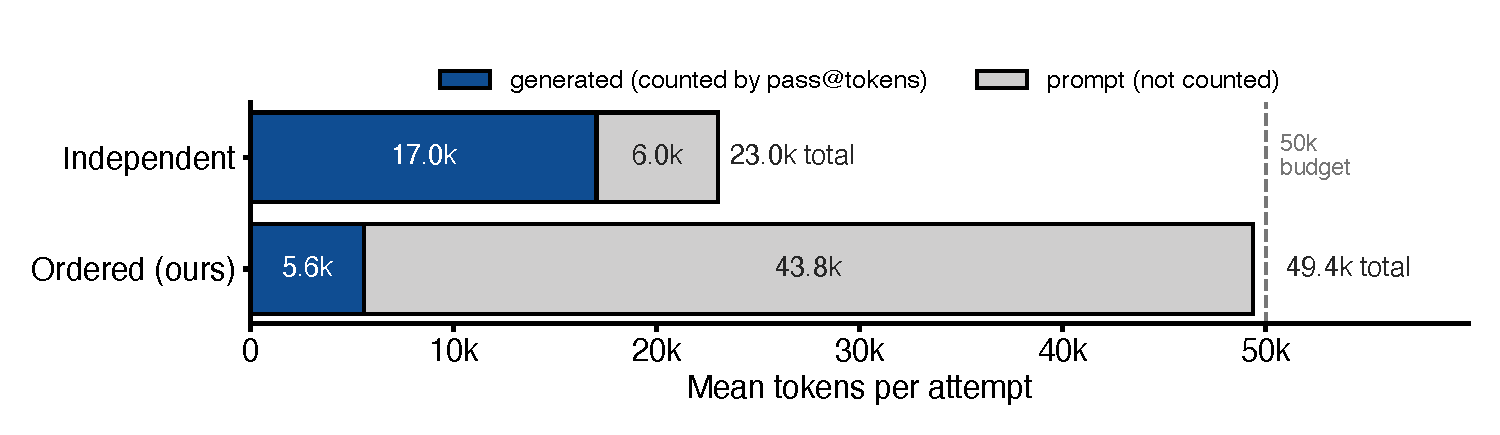
\includegraphics[width=0.85\linewidth]{figures/tokens_per_attempt.pdf}
\caption{Mean tokens per attempt, split into generated tokens (counted by pass@tokens) and input tokens (not counted).
\ordered{} writes a third of \indep's tokens but reads seven times the input. Counting both, a 50k budget buys one
\ordered{} attempt and two \indep{} attempts.}
\label{fig:tokens}
\end{figure}

\paragraph{The saving moves into the input.} The finished code that \ordered{} reuses has to be shown to the model, as
input. An \ordered{} attempt reads 43,779 input tokens against \indep's 5,980 (Figure~\ref{fig:tokens}). Counting input
and generated tokens together, an attempt costs 49.4k against 23.0k. A 50k budget in total tokens then buys one
\ordered{} attempt (0.095) and two \indep{} attempts (0.165), and the order of the two methods reverses.

\paragraph{GPU time.} Input tokens are cheaper than generated ones, so the truth lies between the two counts. Measured
directly, an \ordered{} attempt took 16.4 GPU-seconds and an \indep{} attempt 26.8: 1.6 times cheaper, not three.
\ordered{} generated 340 tokens per second against \indep's 636, because it reads long inputs and builds level by level
in smaller batches. With GPU-seconds as the price (Figure~\ref{fig:budget}(b)), the largest budget both methods cover
is 80 GPU-seconds per problem, and there the difference is $+0.028$ $[-0.006, +0.062]$, an interval that includes zero.
This measure depends on our scheduler; caching shared input across calls, or batching across levels, could narrow the
speed gap.

\paragraph{Coherent programs do the work.} Of \ordered's 212 passing attempts, 197 passed with one of their eight
coherent programs, and in the median attempt the very first program built was the one that passed. Random
recombination, the core of \indep, added little once bodies were written against real code.

% =====================================================================================================================
\section{Reproducing DecompRL's baseline}
\label{sec:harness}

Our pre-registered sanity check failed, and this limits what our absolute numbers mean. \plain{} solves 0.183, 0.283
and 0.312 at 1k, 5k and 10k tokens, where DecompRL reports 0.06, 0.16 and 0.21 for the same untrained model. Our
untrained baseline sits on DecompRL's reinforcement-learning row (GRPO) instead.

We re-scored our saved attempts under other plausible rules after the run (Table~\ref{tab:harness}). DecompRL's stated
rule, with its reported 387 tokens per attempt, does not reproduce its row: our attempts simply pass more often.
Counting the full input in every attempt comes within 0.05 at 5k, 10k and 50k but not at 1k, and the paper says it
counts generated tokens. Platform does not explain the gap: AtCoder and LeetCode problems score alike. The one number
that lines up is untrained hierarchical generation with a single attempt: 11.3\% here, 11.0\% in DecompRL's Table~4.
Without the authors' prompts and accounting we cannot locate the difference. We therefore compare methods only inside
our own setup, where all three share every condition, and never set our absolute scores beside the paper's.

\begin{table}[t]
\centering
\caption{\plain{} re-scored under other budget rules, beside DecompRL's Table~1. An asterisk marks budgets where fewer
than 95\% of problems have enough attempts (scores biased low).}
\label{tab:harness}
\begin{tabular}{lcccc}
\toprule
\plain{}, scored as & 1k & 5k & 10k & 50k \\
\midrule
ours: 260 generated tokens per attempt & 0.183 & 0.283 & 0.312 & 0.312* \\
DecompRL's reported 387 tokens per attempt & 0.160 & 0.260 & 0.295 & 0.312* \\
input counted in every attempt (1,496 per attempt) & 0.122 & 0.183 & 0.223 & 0.306 \\
\midrule
DecompRL Table 1, untrained & 0.06 & 0.16 & 0.21 & 0.30 \\
DecompRL Table 1, GRPO-trained & 0.18 & 0.29 & 0.32 & 0.38 \\
\bottomrule
\end{tabular}
\end{table}

% =====================================================================================================================
\section{Discussion}
\label{sec:discussion}

\paragraph{Report all three costs.} A budget in generated tokens is a natural choice when output dominates the cost,
as it does for long reasoning traces. It is the wrong single number for methods that differ in how much they read.
Any technique that shows the model more context (retrieved code, earlier attempts, finished dependencies) can lower
its generated-token count while raising its true cost. We suggest that budget-based evaluations of code generation
report generated tokens, input tokens and GPU time side by side, and state which one a claim rests on.

\paragraph{What this says about DecompRL.} Little, directly. DecompRL's trained model writes much shorter attempts
than the untrained one (about 4,000 tokens per attempt in its Table~3, against 17,032 here), and training could change
the comparison in either direction. What our results do say is that build order is a real design dimension of
hierarchical generation, with a measurable effect on where the cost of an attempt goes.

\paragraph{Ongoing work: training each method.} We have run one round of self-training per method, in which each
method samples on 1,500 CodeContests training problems~\citep{li2022alphacode}, keeps the samples that pass, and
fine-tunes a low-rank adapter~\citep{dettmers2023qlora} on them~\citep{zelikman2022star, yuan2023rft}. Each method
got the same 1.5 GPU-hours to collect data. \plain{} passed on 1,478 of 8,928 attempts, \indep{} on 22 of 216 and
\ordered{} on 16 of 312: at equal compute, the decomposition methods collect very little training data. The trained
models are being evaluated on a separate development set of 119 newer LiveCodeBench problems; the 279 test problems
will be used once, for a final frozen method.

\paragraph{Limitations.}
\begin{itemize}
  \item Our setup does not reproduce DecompRL's untrained baseline (Section~\ref{sec:harness}); absolute scores are not
        comparable with the paper's.
  \item No method was trained; the reinforcement-learning-trained DecompRL model is not part of this comparison.
  \item One model, one benchmark window and 279 problems; budgets reach 50k tokens, where DecompRL reports up to 500k.
  \item GPU-time results depend on our serving code and on T4 GPUs.
  \item One decomposition per attempt makes each attempt all-or-nothing: a plan with a wrong specification fails every
        program built from it.
\end{itemize}

% =====================================================================================================================
\section{Related work}
\label{sec:related}

\paragraph{Hierarchical and modular code generation.} Parsel~\citep{zelikman2023parsel} has a model describe a program
as a hierarchy of functions, implements each, and searches over combinations of implementations against tests.
CodeChain~\citep{le2024codechain} asks for modular code and revises it by reusing representative sub-modules.
DecompRL~\citep{decugis2026decomprl} trains decomposition and implementation with reinforcement learning, writes
functions independently, and introduces pass@tokens. \ordered{} keeps DecompRL's procedure and changes only the build
order and what each call sees.

\paragraph{Spending compute at inference.} Repeated sampling with a verifier keeps improving coverage as samples grow
\citep{brown2024monkeys}, and how best to spend inference compute depends on the problem and the method
\citep{snell2024scaling}. Our results add that the unit in which that compute is counted can decide which method looks
best.

\paragraph{Training on verified samples.} Self-training on a model's own correct outputs, as in STaR
\citep{zelikman2022star} and rejection-sampling fine-tuning \citep{yuan2023rft}, is a cheap relative of reinforcement
learning and the basis of our ongoing training experiments.

% =====================================================================================================================
\section{Conclusion}

Building functions in dependency order, and showing each function the code it calls, makes hierarchical code
generation solve more problems than DecompRL's independent procedure at a fixed budget of generated tokens. The gain
comes from cheaper attempts, and the saving reappears as input the model must read: in total tokens the order reverses,
and in GPU time the difference is not significant. On an untrained 7B model, plain sampling beats both. Evaluations
that price attempts in generated tokens alone should be read with that blind spot in mind.

\section*{Acknowledgments}
All experiments ran on Kaggle's free GPU tier. The experiment code and a first draft of this paper were written with
the help of an AI assistant (Claude, Anthropic). The author proposed the ordered method, fixed the experimental design
and analysis plan before the main run, and takes responsibility for the content.

\bibliographystyle{plainnat}
\bibliography{refs}

% =====================================================================================================================
\clearpage
\appendix

\section{Prompts}
\label{app:prompts}

\plain{} uses LiveCodeBench's standard code-generation prompt. \indep{} uses DecompRL's decomposition and implementation
prompts (its Appendix~I) verbatim. For LeetCode problems, both decomposition methods append the required function
signature to the problem text; for AtCoder problems, a note that the program reads standard input and writes standard
output. \ordered{} adds the following lines to DecompRL's prompts and changes nothing else.

\paragraph{Added to the decomposition prompt} (and the worked example gains matching \texttt{Uses:} lines):
\begin{lstlisting}
- End each docstring with a line `Uses: name1, name2` naming the component functions it calls,
  or `Uses: -` if it calls none of them.
- List the functions basics first: each function comes after every function it uses.
\end{lstlisting}

\paragraph{Added to the implementation prompt} (functions it uses are shown with finished bodies instead of stubs):
\begin{lstlisting}
- Functions shown with a body are already written; read them and call them as they are.
- If you need a helper function that is in neither list, do not write code that calls it. Instead
  reply with only one line per missing function, in the form
  MISSING: def name(arguments) -> return_type: what it does
  and nothing else. It will be written first, then you will be asked again.
\end{lstlisting}

\paragraph{Helper prompt.} A missing helper is written with DecompRL's implementation prompt, adapted to name the
helper, the reason it is needed, and the decomposition it belongs to.

\section{Settings}
\label{app:settings}

\begin{center}
\begin{tabular}{lr}
\toprule
Setting & Value \\
\midrule
Bodies per function ($k$) & 8 \\
Programs graded per attempt, at most & 128 \\
Functions per decomposition, at most & 6 \\
Tokens per decomposition / per plain program, at most & 2,048 \\
Tokens per function body, at most & 1,024 \\
\texttt{MISSING} rounds per function, at most & 2 \\
Temperature / top-$p$ & 1.0 / 1.0 \\
Context length & 8,192 \\
Time limit per program & $2T+1$ CPU-seconds for $T$ tests \\
Bootstrap resamples & 4,000 \\
Coverage threshold & 95\% of problems \\
\bottomrule
\end{tabular}
\end{center}

\section{Full pass@tokens table}
\label{app:full}

\begin{center}
\begin{tabular}{rcccc}
\toprule
Budget (tokens) & \plain{} & \indep{} & \ordered{} & Attempts $k$, in the same order \\
\midrule
1,000  & 0.183 & 0.113 & 0.095 & 3 / 1 / 1 \\
2,000  & 0.231 & 0.113 & 0.095 & 7 / 1 / 1 \\
4,000  & 0.272 & 0.113 & 0.095 & 15 / 1 / 1 \\
5,000  & 0.283 & 0.113 & 0.095 & 19 / 1 / 1 \\
10,000 & 0.312 & 0.113 & 0.095 & 38 / 1 / 1 \\
20,000 & --    & 0.113 & 0.173 & -- / 1 / 3 \\
30,000 & --    & 0.113 & 0.208 & -- / 1 / 5 \\
40,000 & --    & 0.165 & 0.229 & -- / 2 / 7 \\
50,000 & --    & 0.165 & 0.237 & -- / 2 / 8 \\
\bottomrule
\end{tabular}
\end{center}

\paragraph{A stricter check.} Equation~\eqref{eq:budget} grants at least one whole attempt even when the budget is
smaller than an attempt. Under a stricter rule, which counts an attempt only once all of its tokens fit in the budget
(averaged over random orders of the attempts), \ordered{} minus \indep{} at 10k tokens is $+0.115$ $[+0.085, +0.147]$:
at that budget an \indep{} attempt usually does not fit at all.

\section{Reproducibility}
\label{app:repro}

The repository \url{https://github.com/RatnaAnimesh/build-order-codegen} holds the code, prompts and the main run's
record. The record holds every attempt's token counts,
generation time and test results (not the program text), and all numbers in this paper are computed from it. The
repository's README is the lab log, in which each decision of the analysis plan is dated before the run it governs.

\end{document}
